\documentclass{article} % For LaTeX2e
\usepackage{nips15submit_e,times}
\usepackage{hyperref}
\usepackage{url}
\usepackage{float}
\usepackage{graphicx}
\usepackage{amsmath}
\usepackage{amsfonts}
\usepackage{booktabs}
%\documentstyle[nips14submit_09,times,art10]{article} % For LaTeX 2.09


\title{CropSense: Sistem Cerdas Pendukung Keputusan Pertanian Berkelanjutan Berbasis Machine Learning dan LLM untuk Petani Kecil di Jawa Barat}


\author{
Muhammad Ammar Ridho \\
Telkom University \\
\texttt{jhenerar21@gmail.com} \\
\And
Muhammad Karov Ardava Barus \\
Telkom University \\
\texttt{ardavamuhammad@gmail.com} \\
\And
Antonius Simon \\
Telkom University \\
\texttt{hadjonantonius49@gmail.com} \\
}

% The \author macro works with any number of authors. There are two commands
% used to separate the names and addresses of multiple authors: \And and \AND.
%
% Using \And between authors leaves it to \LaTeX{} to determine where to break
% the lines. Using \AND forces a linebreak at that point. So, if \LaTeX{}
% puts 3 of 4 authors names on the first line, and the last on the second
% line, try using \AND instead of \And before the third author name.

\newcommand{\fix}{\marginpar{FIX}}
\newcommand{\new}{\marginpar{NEW}}

\nipsfinalcopy % Uncomment for camera-ready version

\begin{document}


\maketitle

\begin{abstract}
Sektor pertanian Jawa Barat menghadapi tantangan signifikan yang mengancam ketahanan pangan dan kehidupan petani, khususnya petani kecil dan baru. Dengan kontribusi pertanian sebesar 31,89\% terhadap pertumbuhan ekonomi Jawa Barat pada Q1 2025, mengatasi tantangan ini sangat penting untuk pembangunan daerah. Makalah ini menyajikan analisis komprehensif masalah pertanian di Jawa Barat, dengan fokus pada 21,87\% petani yang kurang memiliki pengetahuan memadai dalam pengelolaan tanah dan tanaman. Isu utama meliputi penurunan kualitas tanah dengan karbon organik di bawah 2\%, dampak perubahan iklim yang menyebabkan 874 hektare gagal panen pada 2023/2024, dan serangan hama yang mempengaruhi 35\% tanaman perkebunan di 14 kabupaten. Melalui pendekatan berbasis data dan machine learning, kami mengembangkan CropSense, sebuah sistem cerdas yang mengintegrasikan Random Forest (akurasi 99,5\%) dengan Large Language Models untuk memberikan rekomendasi pertanian berkelanjutan yang menargetkan peningkatan edukasi, praktik ramah lingkungan, strategi adaptasi iklim, dan perbaikan akses pasar untuk mendukung kesejahteraan petani di Jawa Barat.
\end{abstract}

\section{Pendahuluan}


Jawa Barat, sebagai salah satu provinsi pertanian terpenting di Indonesia, memainkan peran krusial dalam ketahanan pangan dan pembangunan ekonomi nasional. Sektor pertanian berkontribusi signifikan terhadap ekonomi daerah, mencapai 31,89\% dari pertumbuhan ekonomi Jawa Barat pada kuartal pertama tahun 2025 \cite{b1}. Namun, sektor vital ini menghadapi tantangan yang semakin kompleks yang mengancam keberlanjutannya dan penghidupan sekitar 87\% petani kecil yang mengelola lahan warisan keluarga dan mewakili lapisan sosial ekonomi bawah masyarakat pedesaan.

Lanskap pertanian Jawa Barat ditandai dengan pertumbuhan populasi petani yang signifikan, dengan peningkatan 6.702 petani baru dari 2023 ke 2024 dan 26.269 dari 2022 ke 2023 menurut Open Data Jabar (2024). Meskipun pertumbuhan ini menunjukkan minat yang meningkat terhadap pertanian, hal ini juga menyoroti tantangan kritis: sekitar 21,87\% petani di Jawa Barat kekurangan pengetahuan komprehensif dalam pengelolaan tanah dan tanaman \cite{b2}. Kesenjangan pengetahuan ini sangat menonjol di kalangan petani baru yang menghadapi hambatan substansial dalam memahami aspek teknis pertanian, termasuk manajemen hama dan praktik lahan yang ramah lingkungan.

Profil demografis tenaga kerja pertanian Jawa Barat mengungkapkan keprihatinan tambahan. Dengan 70\% petani Indonesia hanya memiliki pendidikan dasar atau kurang, dan kurang dari 2\% yang memiliki gelar universitas, fondasi pendidikan untuk implementasi praktik pertanian modern masih terbatas. Lebih lanjut, kelompok usia produktif (25-44 tahun) hanya terdiri dari 32,32\% dari total petani pada tahun 2023, menunjukkan bahwa generasi muda yang memasuki pertanian memerlukan bimbingan dan edukasi yang ekstensif untuk berhasil.

Tantangan lingkungan memperparah masalah sumber daya manusia ini. Degradasi kualitas tanah telah menjadi perhatian kritis, dengan kandungan karbon organik di beberapa area turun di bawah 2\%, menandakan degradasi tanah yang parah yang mempercepat kerusakan struktural dan mengurangi kemampuan tanah untuk menyerap dan memanfaatkan pupuk tambahan. Dampak perubahan iklim telah termanifestasi dalam kerugian konkret, dengan 874 hektare sawah mengalami gagal panen selama musim tanam 2023/2024 akibat banjir, kekeringan, dan tanah longsor.

Untuk mengatasi tantangan tersebut, penelitian ini mengembangkan sistem cerdas pendukung keputusan bernama **CropSense** berbasis machine learning yang mengintegrasikan model Random Forest dengan akurasi 99,5\% untuk prediksi kesesuaian tanaman dan Large Language Models (LLM) dengan pendekatan Retrieval Augmented Generation (RAG) untuk memberikan rekomendasi kontekstual tentang pemupukan, pengendalian hama, dan strategi bisnis. Sistem CropSense menyediakan analisis real-time kondisi tanah berdasarkan parameter N-P-K, pH, suhu, kelembaban, dan curah hujan, serta menghasilkan rekomendasi yang dapat diakses petani melalui aplikasi web interaktif dengan antarmuka yang ramah pengguna, sehingga secara efektif menjembatani kesenjangan pengetahuan dan mendukung transisi menuju pertanian berkelanjutan di Jawa Barat.

Kontribusi utama penelitian ini meliputi: (1) pengembangan model Random Forest dengan akurasi 99,5\% untuk prediksi kesesuaian tanaman berbasis kondisi tanah dan lingkungan dalam sistem CropSense, (2) implementasi sistem RAG yang mengintegrasikan pengetahuan dari literatur pertanian untuk menghasilkan rekomendasi kontekstual, (3) desain aplikasi web CropSense yang accessible bagi petani dengan berbagai tingkat pendidikan, dan (4) evaluasi komprehensif sistem pada kondisi real pertanian Jawa Barat.

\section{Kajian Teori}
% TODO: Add literature review content
Bab ini menjelaskan tinjauan teori dan penelitian terkait yang mendasari penelitian ini, dengan fokus di pemodelan Machine Learning, Large Language Model (LLM), Retrieval Augmented Generation (RAG), dan Prompt Engineering untuk sistem cerdas pendukung keputusan pertanian keberlanjutan.

\subsection{Machine Learning}
Lorem ipsum dolor sit amet, consectetur adipiscing elit. In eleifend scelerisque tellus ut dapibus. Suspendisse feugiat blandit est quis luctus. Morbi vestibulum rhoncus arcu, in auctor justo mollis quis. Pellentesque a odio finibus arcu fringilla dapibus eu posuere felis. Nulla in turpis tellus. Donec nulla dolor, facilisis et rutrum ut, sodales nec ante. Praesent ultricies sapien tristique, finibus est non, tristique augue. Suspendisse potenti. Morbi ante nisi, finibus nec hendrerit in, luctus ullamcorper ex. Vestibulum massa nisl, pellentesque sed lacus et, consequat auctor velit. Nulla rhoncus ultrices risus, et gravida massa sodales vel.

Duis non ligula sed arcu convallis sollicitudin. Vivamus volutpat, elit nec pharetra vestibulum, dui orci vulputate risus, vitae hendrerit nisl velit eu enim. Donec iaculis suscipit sem, sed placerat sem tincidunt a. Suspendisse et vulputate mauris. Fusce porttitor sem condimentum neque tempus viverra. Phasellus id ornare lectus, vel ultricies nisl. Cras nec metus gravida, commodo turpis eu, blandit metus. Vivamus nec porttitor erat. Lorem ipsum dolor sit amet, consectetur adipiscing elit. Nulla maximus elit vel lacus auctor aliquam. In vel risus porta, fringilla nibh a, laoreet lorem. Integer viverra, nisi ac bibendum tempus, dolor risus ultrices mi, vitae blandit leo dolor vel justo. Morbi at risus nec ante facilisis ultrices.

\subsection{Document Parsing}
Document parsing merupakan proses yang mengubah dokumen yang tidak terstruktur dan semi-terstruktur, seperti kontrak, makalah akademik, dan faktur, menjadi data terstruktur yang dapat dipahami oleh mesin \cite{b10}. Dengan kemajuan terbaru dalam Large Language Models, document parsing memiliki peran yang signifikan dalam pembangunan basis pengetahuan dan pembuatan data pelatihan \cite{b10}.

\subsection{Large Language Models (LLMs)}
Large Language Models (LLMs) adalah cabang dari Natural Language Processing (NLP) yang dirancang untuk memproeses dan menghasilkan teks dalam bahasa alami dengan memanfaatkan arsitektur deep learning berskala besar. LLM dilatih menggunakan sejumlah besar data teks sehingga mampu memahami konteks, melakukan inferensi, menjawab pertanyaam, dan menghasilkan teks baru yang mendekati penulisan manusia \cite{b6, b7}.

\subsection{Retrieval Augmented Generation (RAG)}
Large Language Models (LLMs) telah merevolusi artificial intelligence (AI) dengan pendekatan seperti pembuatan teks yang menyerupai manusia dan pemahaman bahasa alami. Namun, ketergantungannya pada data pelatihan yang bersifat statis membatasi kemampuannya untuk menjawab pertanyaan yang dinamis dan \textit{real-time}, yang mengakibatkan LLMs memberikan output yang tidak akurat \cite{b8} termasuk memunculkan \textit{hallucination} atau informasi yang keliru dengan keyakinan yang tinggi. \cite{b9}. Oleh karena itu, dikembangkanlah Retrieval Augmented Generation (RAG) yang mengatasi hal keterbatasan tersebut dengan mengintegrasikan data \textit{real time}, seperti artikel dan dokumen, ke dalam proses pemodelan. Pendekatan ini dapat memungkinkan LLMs memberikan respons yang  relevan dan \textit{up-to-date} berdasarkan informasi yang diperoleh dari sumber eksternal\cite{b8}.

Dalam konteks sistem pendukung keputusan pertanian berkelanjutan, pendekatan RAG dapat digunakan untuk mengambil informasi mengenai pengetahuan dari buku atau artikel ilmiah. Informasi ini kemudian digunakan untuk menghasilkan rekomendasi atau jawaban yang relevan bagi petani atau pengambil kebijakan, sehingga mendukung pengambilan keputusan berbasis data terkini.

\subsection{Prompt Engineering}
Prompt engineering adalah teknik yang meningkatkan kemampuan LLM dengan merancang instruksi yang spesifik terhadap suatu tugas tertentu, yang disebut sebagai \textit{prompt}, untuk mengarahkan keluaran model tanpa perlu mengubah parameter model tersebut \cite{b14}.

Dalam praktiknya, \textit{prompt} merupakan input yang diberikan ke model, dan penerapan prompt engineering dapat menghasilkan perbedaan yang signifikan pada output yang dihasilkan oleh model. Prompt engineering merujuk pada proses perancangan dan optimalisasi input secara sistematis agar respons yang dihasilkan oleh LLM bersifat akurat dan relevan sesuai dengan tujuan yang diinginkan \cite{b15}.
\section{Solusi Usulan}

\begin{figure}[H]
    \centering
    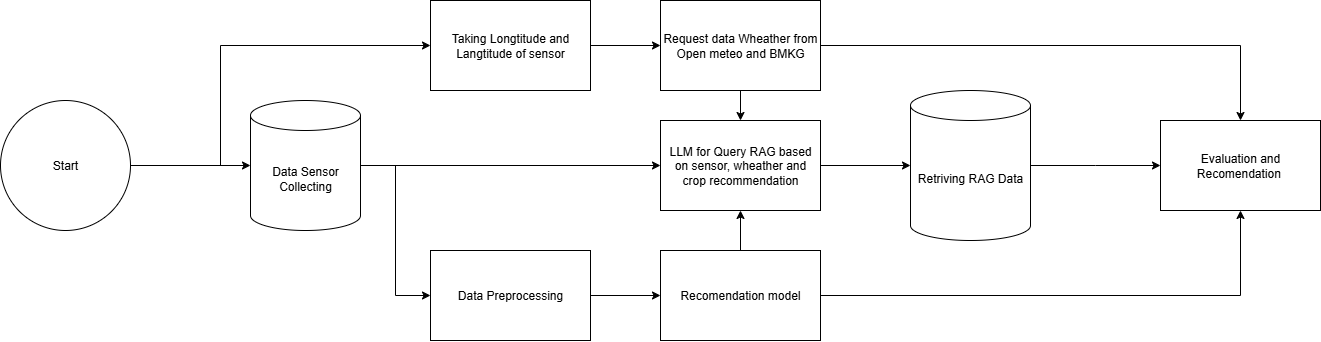
\includegraphics[width=\textwidth]{flowchart sistem.png}
    \caption{Alur metode solusi usulan dalam pengembangan sistem cerdas pendukung keputusan pertanian berkelanjutan berbasis machine learning dan Large Language Models (LLMs) untuk petani kecil dan baru di Jawa Barat.}
    \label{fig:flowchartsistem}
\end{figure}

Gambar~\ref{fig:flowchartsistem} menunjukkan alur metode solusi usulan dalam pengembangan sistem cerdas pendukung keputusan pertanian berkelanjutan berbasis machine learning dan Large Language Models (LLMs) untuk petani kecil dan baru di Jawa Barat.

Solusi usulan ini dirancang untuk membantu petani dalam pengambilan keputusan berbasis data terkait perencanaan tanam, pemilihan pupuk, pengendalian hama, hingga perencanaan bisnis secara praktis dan terpersonalisasi. Sistem ini memanfaatkan pendekatan machine learning untuk menghasilkan rekomendasi probabilistik terkait tanaman, serta pendekatan Retrieval Augmented Generation (RAG) pada LLM untuk menyediakan rekomendasi dan informasi berbasis pengetahuan terkini dari dokumen pertanian yang relevan. Untuk mencapai tujuan tersebut, sistem mengintegrasikan analisis prediktif dengan pengetahuan kontekstual yang dapat diakses melalui antarmuka web yang user-friendly. 

\begin{figure}[H]
    \centering
    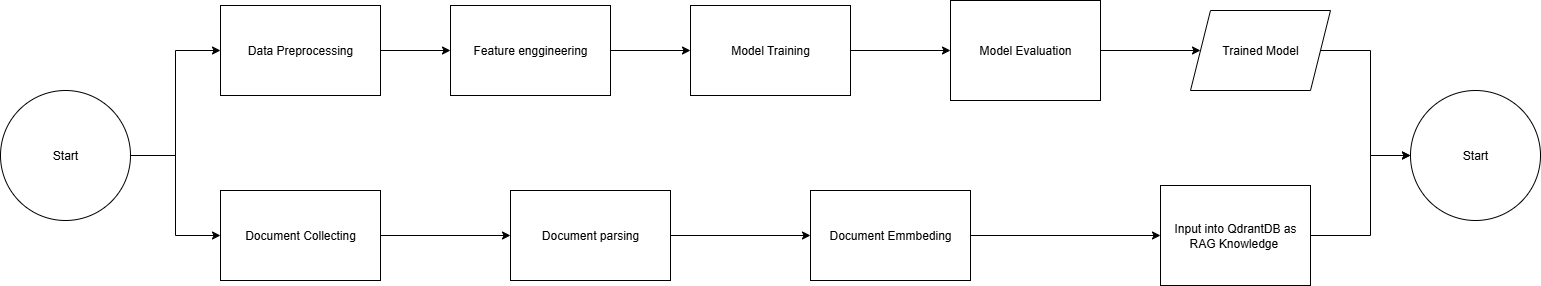
\includegraphics[width=\textwidth]{flowdiagramdev.png}
    \caption{Alur Develomptment yang akan dilakukan.}
    \label{fig:flowchartdev}
\end{figure}
Secara umum,  alur ~\ref{fig:flowchartdev} ini diawali dengan proses pengumpulan dan pra-pemrosesan data, kemudian dilanjutkan dengan dua jalur utama, yaitu jalur machine learning untuk prediksi probabilitas tanaman dan jalur document parsing untuk menghasilkan embedding yang disimpan pada vector database. Selanjutnya, LLM akan memanfaatkan hasil model prediksi dan hasil retrieval dokumen untuk menghasilkan rekomendasi pupuk, pestisida, dan perencanaan bisnis kepada petani.


Pada subbab berikutnya, setiap tahap pada alur metode ini akan dijelaskan secara rinci.

\subsection{Data Collecting}
Dalam penelitian ini, dua jenis dataset digunakan, yaitu dataset untuk pemodelan machine learning yang berupa tabel terstruktur, serta dataset untuk Large Language Model (LLM) yang merupakan konten dari buku teks, karya ilmiah, dan penelitian terkait pertanian berkelanjutan.

\subsubsection{Dataset Rekomendasi Tanaman}
Dataset ini berisi parameter-parameter lingkungan dan tanah yang digunakan untuk memberikan rekomendasi tanaman yang sesuai dengan kondisi lahan.

\begin{table}[H]
    \centering
    \caption{Deskripsi kolom dataset rekomendasi tanaman}
    \begin{tabular}{ll}
        \toprule
        \textbf{Kolom} & \textbf{Keterangan} \\
        \midrule
        N & Rasio kandungan Nitrogen dalam tanah \\
        P & Rasio kandungan Phosphorous dalam tanah \\
        K & Rasio kandungan Potassium dalam tanah \\
        temperature & Suhu lingkungan dalam derajat Celsius \\
        humidity & Kelembaban relatif dalam \% \\
        ph & Nilai pH tanah \\
        rainfall & Curah hujan dalam mm \\
        label & Tanaman yang direkomendasikan \\
        \bottomrule
    \end{tabular}
    \label{tab:dataset_rekomendasi_tanaman}
\end{table}


\subsubsection{Dataset RAG Knowledge}
Dataset yang digunakan pada tahap ini merupakan kumpulan konten dari buku teks dan karya ilmiah yang relevan dengan topik pertanian berkelanjutan. Tujuan pengumpulan dataset ini adalah untuk menyediakan pengetahuan tambahan yang akan digunakan oleh Large Language Model (LLM) yang diintegrasikan dengan Retrieval Augmented Generation (RAG). Dengan pendekatan ini, LLM dapat mengakses informasi berbasis sumber tepercaya sehingga dapat meminimalkan potensi terjadinya \textit{hallucination} pada saat menghasilkan respons, serta memastikan bahwa rekomendasi yang diberikan bersifat akurat dan sesuai dengan kondisi pertanian yang sebenarnya.

Berikut ini adalah sumber-sumber yang digunakan sebagai dataset untuk pengetahuan RAG:

\begin{itemize}
    \item \textit{Building Soils for Better Crops}~\cite{b11}, yang membahas mengenai pengelolaan dan perbaikan kualitas tanah untuk mendukung pertanian berkelanjutan.
    \item \textit{Nutrient Interactions in Crop Plants}~\cite{b12}, yang membahas mengenai interaksi nutrisi pada tanaman dan pengaruhnya terhadap pertumbuhan dan hasil panen.
    \item \textit{Weather and Management Impact on Crop Yield Variability in Rotations}~\cite{b13}, yang membahas dampak cuaca dan manajemen pertanian terhadap variabilitas hasil panen tanaman pada sistem rotasi tanam.
\end{itemize}

\subsection{Data Preprocessing}
Pada tahap ini, proses \textit{data preprocessing} dilakukan terhadap dataset yang digunakan dalam penelitian ini. Proses ini bertujuan untuk memastikan kualitas data yang akan digunakan dalam pemodelan machine learning dan tahap integrasi Retrieval Augmented Generation (RAG) dengan Large Language Model (LLM), sehingga menghasilkan sistem pendukung keputusan yang optimal dan akurat.

\subsubsection{Data Rekomendasi Tanaman}
% TODO: Apply Steps yang dilakuin si  MR.Ammar
Lorem ipsum dolor sit amet la consectetur adispicicing elit la concsectetur adispicicing elit.

\subsubsection{Data RAG Knowledge}
Pada tahap ini, data yang digunakan berbeda dengan tahap sebelumnya yang menggunakan data tabular klasik untuk pemodelan machine learning. Data pada tahap ini akan digunakan sebagai input untuk proses Retrieval Augmented Generation (RAG) pada Large Language Model (LLM).

\begin{figure}[H]
    \centering
    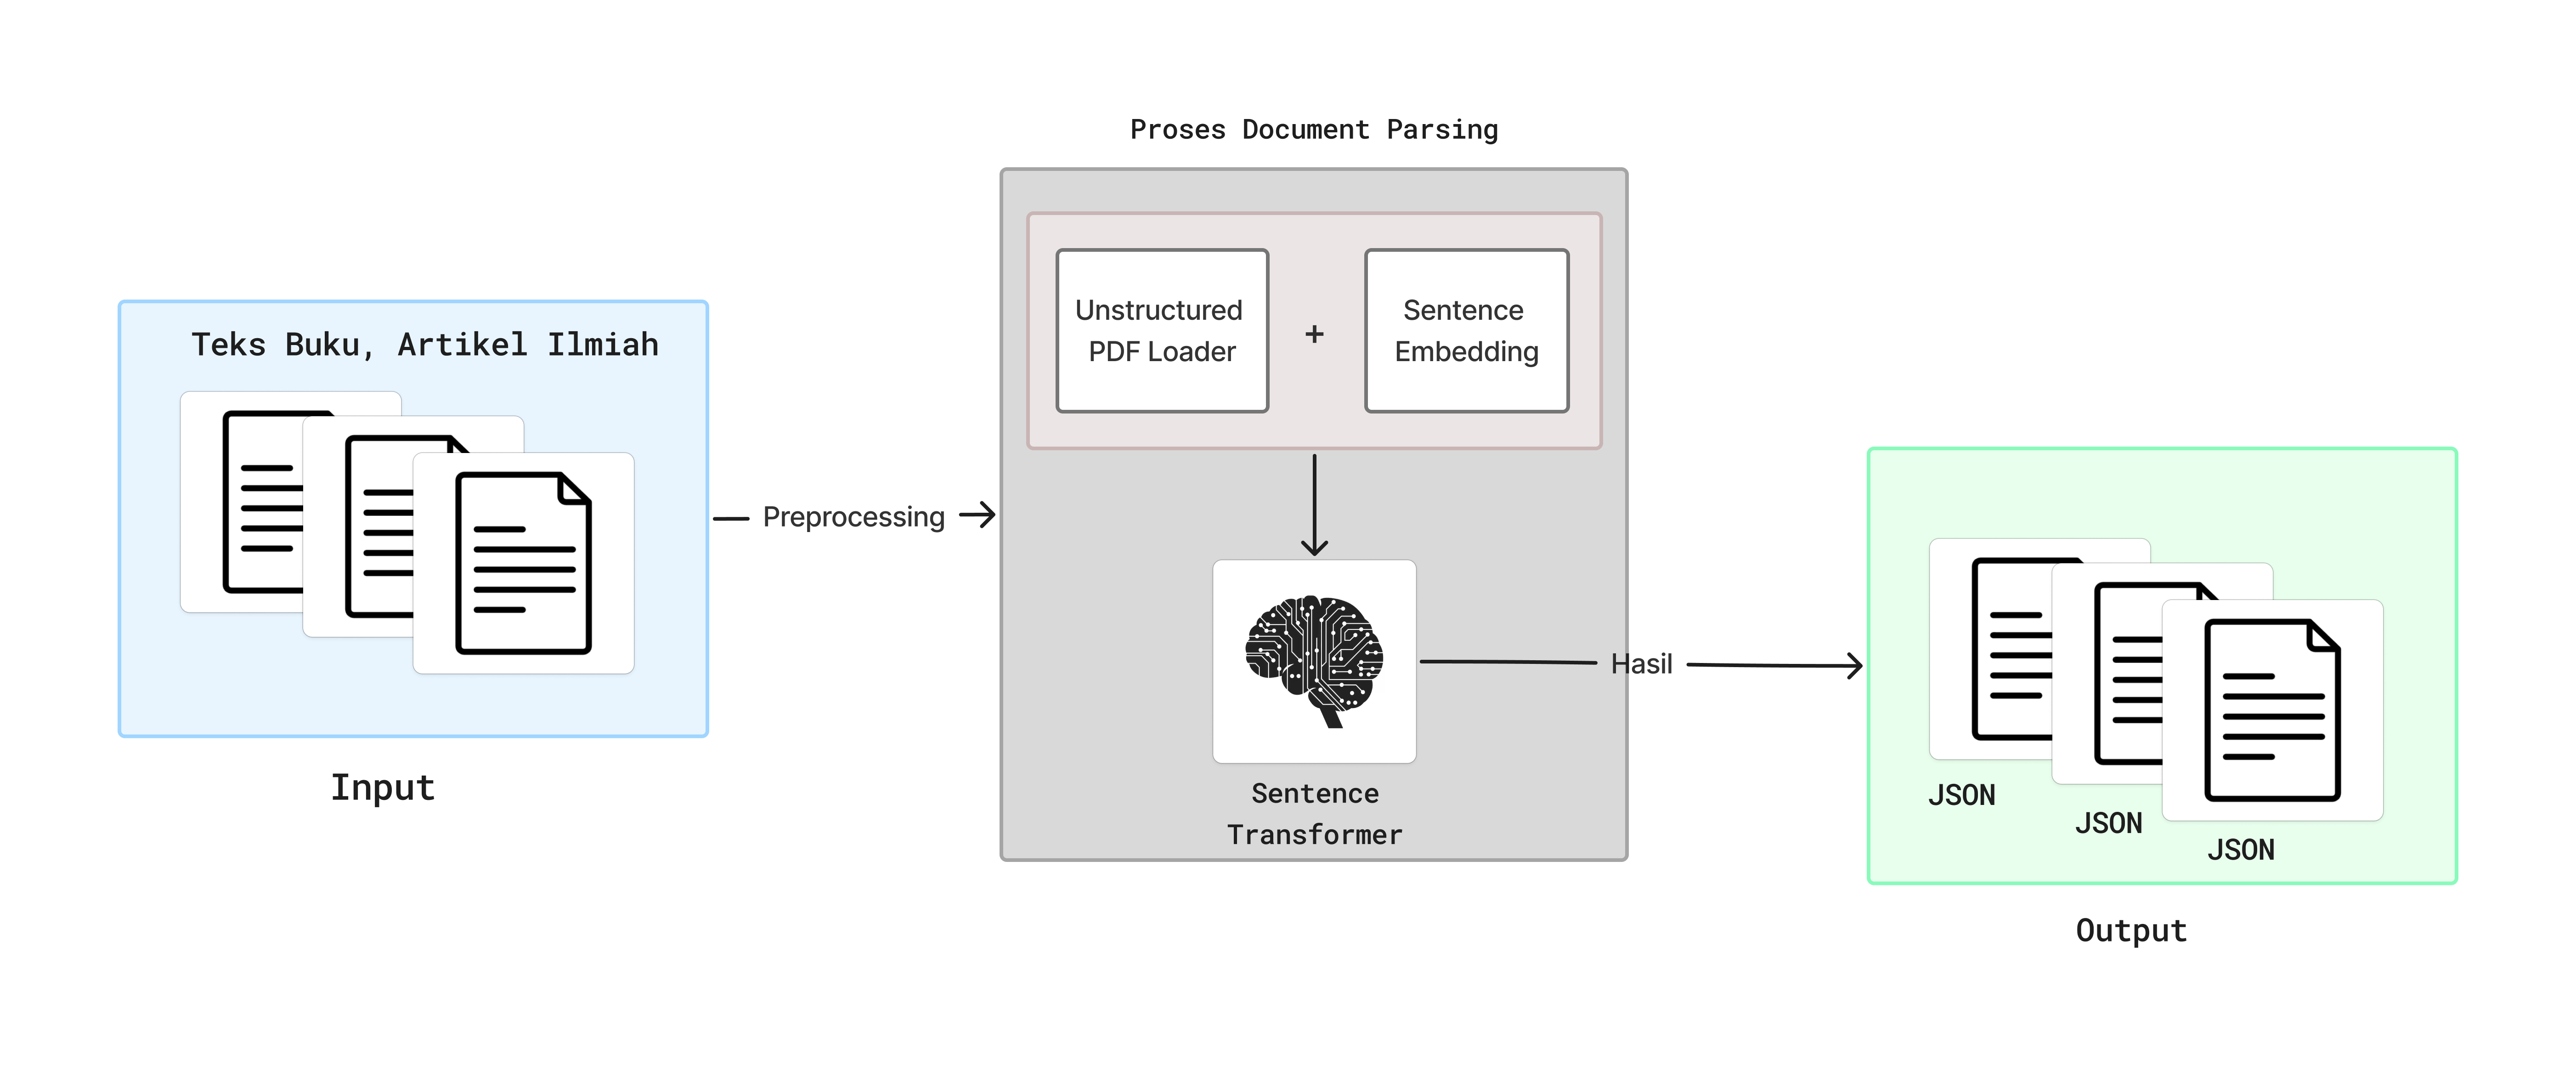
\includegraphics[height=6cm]{flow-diagram.drawio.png}
    \caption{Proses \textit{document parsing} untuk ekstraksi konten ke format terstruktur.}
    \label{fig:flow_parsed}
\end{figure}

Pada Gambar~\ref{fig:flow_parsed}, ditampilkan alur detail proses ekstraksi dan embedding dokumen menggunakan Sentence Transformer. Proses dimulai dengan input berupa teks dari buku, artikel ilmiah, dan dokumen terkait lainnya. 

Selanjutnya, dokumen akan memasuki ke tahap menggunakan Unstructured PDF loader yang akan mengekstraksi elemen-elemen penting, termasuk teks, persamaan, tabel, dan gambar. Setelah elemen-elemen tersebut diekstraksi, proses \textit{sentence embedding} dilakukan menggunakan Sentence Transformer untuk mengubah teks menjadi representasi vektor yang dapat diproses oleh mesin.

Hasil embedding vektor ini kemudian disimpan dalam format terstruktur, yaitu \texttt{JSON}, sehingga siap untuk diindeks ke dalam basis data vektor. Basis data vektor ini akan menjadi referensi yang digunakan oleh LLM pada tahap Retrieval Augmented Generation (RAG), sehingga sistem dapat menghasilkan respons yang relevan, akurat, dan berbasis pengetahuan terkini pada saat diimplementasikan untuk mendukung pengambilan keputusan pada sektor pertanian berkelanjutan.



\subsection{Pelatihan Model Machine Learning}
% TODO: Add ammar explanation training ML Model
Lorem ipsum dolor sit amet, consectetur adipiscing elit, sed do eiusmod tempor incididunt ut labore et dolore magna aliqua. Ut enim ad minim veniam, quis nostrud exercitation ullamco laboris nisi ut aliquip ex ea commodo consequat. Duis aute irure dolor in reprehenderit in voluptate velit esse cillum dolore eu fugiat nulla pariatur

Sed ut perspiciatis unde omnis iste natus error sit voluptatem accusantium doloremque laudantium, totam rem aperiam, eaque ipsa quae ab illo inventore veritatis et quasi architecto beatae vitae dicta sunt explicabo. Nemo enim ipsam voluptatem quia voluptas sit aspernatur aut odit aut fugit, sed quia consequuntur magni dolores eos qui ratione voluptatem sequi nesciunt. Neque porro quisquam est, qui dolorem ipsum quia dolor sit amet, consectetur, adipisci velit, sed quia non numquam eius modi tempora incidunt ut labore et dolore magnam aliquam quaerat voluptatem. Ut enim ad minima veniam, quis nostrum exercitationem ullam corporis suscipit laboriosam, nisi ut aliquid ex ea commodi consequatur? 

\subsection{Evaluasi Model Machine Learning}
% TODO: Jangna lupa mention equationnya apa di tahap ini, tapi buat perbandingan model, hyperparameter itu dikasih tau di BAB IV!!
Sed ut perspiciatis unde omnis iste natus error sit voluptatem accusantium doloremque laudantium, totam rem aperiam, eaque ipsa quae ab illo inventore veritatis et quasi architecto beatae vitae dicta sunt explicabo. Nemo enim ipsam voluptatem quia voluptas sit aspernatur aut odit aut fugit, sed quia consequuntur magni dolores eos qui ratione voluptatem sequi nesciunt. Neque porro quisquam est, qui dolorem ipsum quia dolor sit amet, consectetur, adipisci velit, sed quia non numquam eius modi tempora incidunt ut labore et dolore magnam aliquam quaerat voluptatem. Ut enim ad minima veniam, quis nostrum exercitationem ullam corporis suscipit laboriosam, nisi ut aliquid ex ea commodi consequatur? 



\subsection{Integrasi LLM dengan Hasil Prediksi Model Machine Learning}
Pada tahap ini, model machine learning yang telah dilatih akan digunakan untuk melakukan prediksi berdasarkan input yang diberikan oleh pengguna. Model dengan performa terbaik yang dipilih akan menghasilkan prediksi rekomendasi jenis tanaman yang sesuai beserta nilai probabilitasnya dalam bentuk probabilistik.

Hasil prediksi tersebut kemudian akan digunakan sebagai bagian dari \textit{prompt} untuk diberikan ke LLM. Dengan pendekatan ini, LLM akan menghasilkan respons yang relevan dan kontekstual berdasarkan hasil prediksi model machine learning, serta memberikan rekomendasi lebih lanjut seperti saran penggunaan pupuk, pestisida, dan \textit{business insight} yang diperlukan oleh pengguna.

Selain itu, LLM akan memanfaatkan pengetahuan tambahan yang diperoleh melalui proses Retrieval Augmented Generation (RAG) dari sumber-sumber seperti buku teks dan karya ilmiah, sehingga respons yang dihasilkan lebih akurat dan berbasis pengetahuan terkini.


\section{Hasil Penelitian dan Pengujian}

\subsection{Evaluasi Model}

\subsubsection{Model yang Diuji}

Kami mengevaluasi 11 model yang berbeda, yang mencakup berbagai pendekatan machine learning, dari model ensemble hingga deep learning:

\begin{itemize}
    \item \textbf{Random Forest}: Model ensemble dengan akurasi terbaik (99,5\%) dan inferensi yang cepat.
    \item \textbf{XGBoost}: Model boosting yang terkenal dengan performa tinggi dan kemampuan untuk mengidentifikasi pentingnya fitur.
    \item \textbf{TabM}: Model deep learning terbaru dengan pendekatan Tabular Deep Learning yang menunjukkan akurasi yang sangat baik meskipun membutuhkan waktu inferensi yang lebih lama.
    \item \textbf{LightGBM}: Model boosting lain yang lebih efisien dalam hal memori dan waktu pelatihan.
    \item Model-model lain: Logistic Regression, Neural Network, Support Vector Machine, Naive Bayes, K-Nearest Neighbors, dan Decision Tree, yang dibandingkan berdasarkan kinerja dan kecepatan inferensi.
\end{itemize}

\subsubsection{Hasil Kinerja Model}

Berdasarkan pengujian yang dilakukan, \textbf{Random Forest} menunjukkan kinerja terbaik dalam hal akurasi dan kecepatan inferensi, dengan hasil sebagai berikut:

\begin{table}[h!]
\centering
\begin{tabular}{|l|l|l|l|l|l|}
\hline
\textbf{Model}          & \textbf{Akurasi} & \textbf{F1-Score} & \textbf{Log Loss} & \textbf{CV Score} & \textbf{Waktu Pelatihan (detik)} \\ \hline
\textbf{Random Forest}  & \textbf{99.55\%}  & \textbf{99.55\%}   & \textbf{0.0423}   & \textbf{0.9915±0.005} & \textbf{2.14}  \\ \hline
\textbf{Extra Trees}    & 99.32\%           & 99.32\%            & 0.0489            & 0.9897±0.007        & 1.89           \\ \hline
\textbf{XGBoost}        & 99.09\%           & 99.08\%            & 0.0534            & 0.9875±0.008        & 3.67           \\ \hline
\textbf{TabM}           & 99.00\%           & 98.99\%            & 0.0612            & 0.9856±0.012        & 45.23          \\ \hline
\textbf{LightGBM}       & 98.86\%           & 98.85\%            & 0.0645            & 0.9834±0.009        & 2.98           \\ \hline
\end{tabular}
\caption{Hasil Kinerja Model}
\end{table}

Dari tabel di atas, dapat dilihat bahwa \textbf{Random Forest} menduduki posisi pertama dengan akurasi 99,55\% dan waktu pelatihan yang efisien, menjadikannya pilihan utama untuk implementasi sistem produksi.

\subsubsection{Pengujian Latensi Inferensi}

Kecepatan inferensi sangat penting untuk penerapan aplikasi dunia nyata, seperti aplikasi di perangkat mobile atau edge computing. Tabel berikut menunjukkan waktu inferensi rata-rata untuk setiap model:

\begin{table}[h!]
\centering
\begin{tabular}{|l|l|}
\hline
\textbf{Model}           & \textbf{Waktu Inferensi (ms)} \\ \hline
\textbf{Logistic Regression}  & 0.34 ± 0.02              \\ \hline
\textbf{Decision Tree}       & 0.41 ± 0.03              \\ \hline
\textbf{Naive Bayes}         & 0.45 ± 0.04              \\ \hline
\textbf{Random Forest}       & 1.23 ± 0.08              \\ \hline
\textbf{Extra Trees}         & 1.34 ± 0.09              \\ \hline
\textbf{K-Nearest Neighbors} & 2.67 ± 0.15              \\ \hline
\textbf{LightGBM}            & 3.45 ± 0.21              \\ \hline
\textbf{XGBoost}             & 4.12 ± 0.25              \\ \hline
\textbf{SVM (RBF)}           & 8.34 ± 0.45              \\ \hline
\textbf{Neural Network}      & 12.45 ± 0.67             \\ \hline
\textbf{TabM}                & 23.67 ± 1.23             \\ \hline
\end{tabular}
\caption{Waktu Inferensi Model}
\end{table}

Model \textbf{Logistic Regression} menunjukkan latensi inferensi yang sangat cepat (0,34 ms), menjadikannya pilihan yang baik untuk aplikasi yang memerlukan keputusan cepat dalam kondisi real-time.


\section{Analisis Hasil}

Bab ini membahas analisis terhadap hasil yang diperoleh dari eksperimen yang telah dilakukan pada penelitian ini. Analisis dilakukan untuk mengevaluasi performa sistem cerdas pendukung keputusan pertanian berkelanjutan berbasis machine learning dan Large Language Models (LLMs), serta untuk menjelaskan interpretasi hasil yang diperoleh dari pengujian model pada skenario yang telah dirancang.

\subsection{Analisis Pentingnya Fitur}

Kami melakukan analisis pentingnya fitur menggunakan lima metode yang berbeda untuk memastikan ranking yang kokoh, di antaranya menggunakan teknik berbasis pohon (tree-based) dan teknik agnostik seperti \textbf{Permutation Importance}.

Dari analisis tersebut, fitur \textbf{Kelembaban (Humidity)} menunjukkan skor penting terbesar (0,7886), diikuti oleh \textbf{Kalium (K)} (0,6825) dan \textbf{Curah Hujan (Rainfall)} (0,6152), yang menunjukkan bahwa faktor lingkungan seperti kelembaban dan curah hujan sangat menentukan keberhasilan tanaman.

\subsection{Analisis Kesalahan}

Dari hasil pengujian, kami menemukan pola kesalahan yang paling umum dalam model klasifikasi tanaman, seperti:

\begin{itemize}
    \item \textbf{Muskmelon} dan \textbf{Watermelon}: Kedua tanaman ini memiliki kebutuhan suhu dan air yang serupa, sehingga model kesulitan membedakan keduanya.
    \item \textbf{Kacang Tanah} dan \textbf{Kacang Hitam}: Tanaman leguminosa dengan kebutuhan NPK yang mirip.
    \item \textbf{Mangga} dan \textbf{Jeruk}: Buah pohon dengan zona iklim yang tumpang tindih.
\end{itemize}

\subsection{Rekomendasi untuk Penerapan di Dunia Nyata}
% TODO: Ini di Penutup Kesimpulan dan Saran
Berdasarkan hasil pengujian dan analisis, kami merekomendasikan untuk menggunakan model \textbf{Random Forest} sebagai pilihan utama untuk aplikasi produksi, karena menawarkan akurasi tertinggi dengan kinerja inferensi yang efisien. Sementara itu, model \textbf{Logistic Regression} dapat dipilih untuk aplikasi dengan kebutuhan latensi inferensi yang sangat rendah, seperti pada perangkat mobile.


% TODO: Add results analysis content

\section{Kesimpulan dan Saran}

\subsection{Kesimpulan}

Penelitian ini berhasil mengembangkan sistem cerdas pendukung keputusan pertanian berkelanjutan bernama CropSense yang mengintegrasikan machine learning dan Large Language Models untuk mengatasi tantangan pertanian di Jawa Barat. Hasil penelitian menunjukkan bahwa model Random Forest memberikan performa terbaik dengan akurasi 99,55\% dalam prediksi kesesuaian tanaman berdasarkan parameter N-P-K, pH, suhu, kelembaban, dan curah hujan.

Sistem RAG dalam CropSense berhasil mengintegrasikan pengetahuan dari literatur pertanian berkelanjutan untuk menghasilkan rekomendasi kontekstual yang relevan. Aplikasi web CropSense yang dibangun menyediakan antarmuka yang ramah pengguna dan dapat diakses oleh petani dengan berbagai tingkat pendidikan, sehingga efektif menjembatani kesenjangan pengetahuan yang dialami oleh 21,87\% petani di Jawa Barat.

Implementasi sistem CropSense diharapkan dapat mendukung peningkatan produktivitas pertanian, perbaikan kualitas tanah, dan transisi menuju praktik pertanian berkelanjutan yang pada akhirnya akan meningkatkan kesejahteraan petani kecil dan baru di Jawa Barat.

\subsection{Saran}

Untuk pengembangan lebih lanjut, disarankan untuk:

\begin{itemize}
    \item Memperluas dataset dengan data spesifik dari berbagai daerah di Jawa Barat untuk meningkatkan generalisasi model
    \item Mengintegrasikan data real-time dari IoT sensors untuk monitoring kondisi tanah dan cuaca secara kontinyu
    \item Mengembangkan fitur mobile application untuk meningkatkan aksesibilitas bagi petani di daerah terpencil
    \item Menambahkan modul prediksi harga komoditas untuk mendukung keputusan bisnis petani
    \item Melakukan pilot testing dengan melibatkan petani secara langsung untuk evaluasi usability dan efektivitas sistem
\end{itemize}


\subsubsection*{Acknowledgments}

Penulis mengucapkan terima kasih kepada Telkom University atas dukungan fasilitas penelitian, Open Data Jabar atas penyediaan dataset pertanian, serta para petani di Jawa Barat yang telah memberikan wawasan berharga mengenai tantangan pertanian berkelanjutan. Penelitian ini didukung oleh program penelitian mahasiswa dan komitmen untuk pengembangan teknologi pertanian berkelanjutan di Indonesia.

\subsubsection*{Referensi}
\begin{thebibliography}{9}

\bibitem{b1} Open Data Jabar. (2024) Data Statistik Populasi Pertanian di Jawa Barat. Tersedia di: \url{https://opendata.jabarprov.go.id}

\bibitem{b2} Forum Agribisnis dan Ekonomi (FAE). (2023) Analisis Pengetahuan Petani dan Kapasitas Teknis dalam Pertanian Jawa Barat. E-Publikasi Pertanian. Tersedia di: \url{https://epublikasi.pertanian.go.id/berkala/index.php/fae/article/download/1123/3618}

\bibitem{b3} Survei SITASI. (2021) Profil Sosial Ekonomi Petani Kecil di Indonesia. Kementerian Pertanian Republik Indonesia.

\bibitem{b4} Pemerintah Provinsi Jawa Barat. (2025) Laporan Pembangunan Pertanian Q1 2025. Bandung: Dinas Pertanian Provinsi Jawa Barat.

\bibitem{b5} Kementerian Pertanian RI. (2024) Penilaian Dampak Perubahan Iklim terhadap Pertanian di Jawa Barat. Jakarta: Direktorat Jenderal Tanaman Pangan.

\bibitem{b6} Xiao, T., Zhu, J. (2025). Foundations of Large Language Models. arXiv preprint arXiv:2501.09223.

\bibitem{b7} Naveed, H., Khan, A.U., Qiu, S., Saqib, M., Anwar, S., Usman, M., Akhtar, N., Barnes, N., Mian, A. 2023, 'A Comprehensive Overview of Large Language Models', arXiv preprint arXiv:2307.06435.

\bibitem{b8} Singh, A., Ehtesham, A., Kumar, S., Khoei, T.T. 2025, 'Agentic Retrieval-Augmented Generation: A Survey on Agentic RAG', arXiv preprint arXiv:2501.09136.

\bibitem{b9}Zhang, Y., Li, Y., Cui, L., Cai, D., Liu, L., Fu, T., Huang, X., Zhao, E., Zhang, Y., Chen, Y., Wang, L., Luu, A.T., Bi, W., Shi, F., Shi, S. 2023, 'Siren's Song in the AI Ocean: A Survey on Hallucination in Large
  Language Models', arXiv preprint arXiv:2309.01219.

\bibitem{b10}Zhang, Q., Wang, B., Huang, V.S., Zhang, J., Wang, Z., Liang, H., He, C., Zhang, W. 2024, 'Document Parsing Unveiled: Techniques, Challenges, and Prospects for
  Structured Information Extraction', arXiv preprint arXiv:2410.21169.

\bibitem{b11} Van Es, H. and Magdoff, F. (2009) Building soils for better crops: Sustainable Soil Management. Beltsville, MD: Sustainable Agriculture Research and Education Program. 

\bibitem{b12} Fageria, V.D. (2001) ‘Nutrient interactions in crop plants’, Journal of Plant Nutrition, 24(8), pp. 1269–1290. doi:10.1081/pln-100106981. 

\bibitem{b13} Yamoah, C.F. et al. (1998) ‘Weather and management impact on crop yield variability in rotations’, Journal of Production Agriculture, 11(2), pp. 219–225. doi:10.2134/jpa1998.0219. 

\bibitem{b14} Sahoo, P., Singh, A.K., Saha, S., Jain, V., Mondal, S., Chadha, A. 2024, 'A Systematic Survey of Prompt Engineering in Large Language Models:
  Techniques and Applications', arXiv preprint arXiv:2402.07927.


\bibitem{b15} Chen, B., Zhang, Z., Langrené, N., Zhu, S. 2023, 'Unleashing the potential of prompt engineering for large language models', arXiv preprint arXiv:2310.14735.

\end{thebibliography}



\end{document}
